\documentclass{article}
\usepackage{tikz}
\usepackage{pgfplots}
\pgfplotsset{compat=1.18}
\usepgfplotslibrary{fillbetween}

\begin{document}

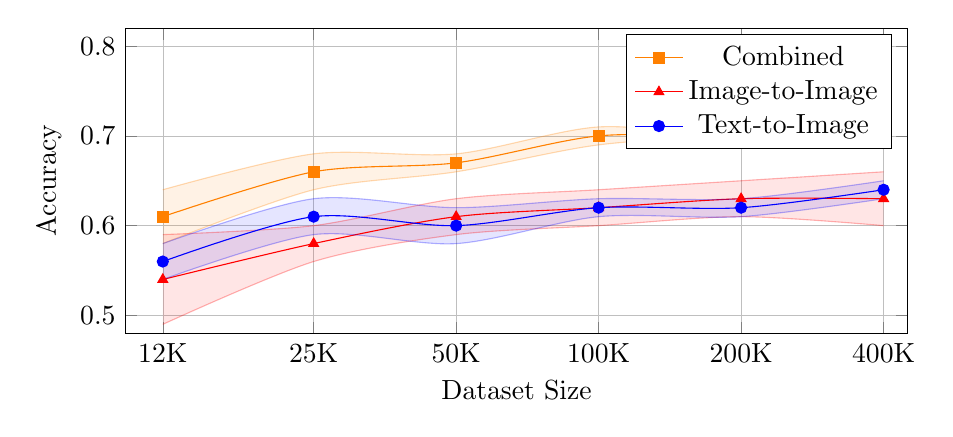
\begin{tikzpicture}
    \centering
    \begin{axis}[
        width=0.95\textwidth,
        height=0.45\textwidth,
        xlabel=Dataset Size,
        ylabel=Accuracy,
        xmode=log,
        xmin=10000, xmax=450000,
        xtick={12000, 25000, 50000, 100000, 200000, 400000},
        xticklabels={12K, 25K, 50K, 100K, 200K, 400K},
        ymin=0.48, ymax=0.82,
        ytick={0.5, 0.6, 0.7, 0.8},
        grid=both,
        major grid style={line width=.2pt,draw=gray!50},
    ]
        \addplot[smooth,color=orange,mark=square*] plot coordinates {
            (12000, 0.61)
            (25000, 0.66)
            (50000, 0.67)
            (100000, 0.7)
            (200000, 0.7)
            (400000, 0.71)
            };
        \addlegendentry{Combined}
        \addplot[smooth, opacity=0.3, name path=TTI1,color=orange,forget plot] plot coordinates {
            (12000, 0.58)
            (25000, 0.64)
            (50000, 0.66)
            (100000, 0.69)
            (200000, 0.7)
            (400000, 0.7)
        };
        \addplot[smooth, opacity=0.3, name path=TTI2,color=orange,forget plot] plot coordinates {
            (12000, 0.64)
            (25000, 0.68)
            (50000, 0.68)
            (100000, 0.71)
            (200000, 0.7)
            (400000, 0.72)
        };
        \addplot[color=orange, opacity=0.4, fill opacity=0.1, forget plot] fill between[of=TTI1 and TTI2];

        \addplot[smooth,mark=triangle*,color=red] plot coordinates {
            (12000, 0.54)
            (25000, 0.58)
            (50000, 0.61)
            (100000, 0.62)
            (200000, 0.63)
            (400000, 0.63)
        };
        \addlegendentry{Image-to-Image}
        \addplot[smooth, opacity=0.3, name path=TTI1,color=red,forget plot] plot coordinates {
            (12000, 0.49)
            (25000, 0.56)
            (50000, 0.59)
            (100000, 0.60)
            (200000, 0.61)
            (400000, 0.60)
        };
        \addplot[smooth, opacity=0.3, name path=TTI2,color=red,forget plot] plot coordinates {
            (12000, 0.59)
            (25000, 0.60)
            (50000, 0.63)
            (100000, 0.64)
            (200000, 0.65)
            (400000, 0.66)
        };
        \addplot[color=red, opacity=0.4, fill opacity=0.1, forget plot] fill between[of=TTI1 and TTI2];
        
        \addplot[smooth,color=blue,mark=*] plot coordinates {
            (12000, 0.56)
            (25000, 0.61)
            (50000, 0.60)
            (100000, 0.62)
            (200000, 0.62)
            (400000, 0.64)
        };
        \addlegendentry{Text-to-Image}
        \addplot[smooth, opacity=0.3, name path=TTI1,color=blue,forget plot] plot coordinates {
            (12000, 0.58)
            (25000, 0.63)
            (50000, 0.62)
            (100000, 0.63)
            (200000, 0.63)
            (400000, 0.65)
        };
        \addplot[smooth, opacity=0.3, name path=TTI2,color=blue,forget plot] plot coordinates {
            (12000, 0.54)
            (25000, 0.59)
            (50000, 0.58)
            (100000, 0.61)
            (200000, 0.61)
            (400000, 0.63)
        };
        \addplot[color=blue, opacity=0.4, fill opacity=0.1, forget plot] fill between[of=TTI1 and TTI2];
        
    \end{axis}
\end{tikzpicture}

\end{document}